% Created 2018-01-30 Tue 11:36
\documentclass[11pt]{article}
\usepackage[utf8]{inputenc}
\usepackage[T1]{fontenc}
\usepackage{fixltx2e}
\usepackage{graphicx}
\usepackage{longtable}
\usepackage{float}
\usepackage{wrapfig}
\usepackage{rotating}
\usepackage[normalem]{ulem}
\usepackage{amsmath}
\usepackage{textcomp}
\usepackage{marvosym}
\usepackage{wasysym}
\usepackage{amssymb}
\usepackage{hyperref}
\tolerance=1000
\usepackage{minted}
\usepackage{float}
\newcommand{\aDE}[4]{\begin{center}\begin{equation}\label{#4}\frac{{dy(t)}}{{dt}} -#1y(t) = #2u(t),y(0) = #3 \end{equation}\end{center}}
\author{Changyuan Lin}
\date{\today}
\title{Test}
\hypersetup{
  pdfkeywords={},
  pdfsubject={},
  pdfcreator={Emacs 25.3.1 (Org mode 8.2.10)}}
\begin{document}

\maketitle
\tableofcontents



\section{Chapter 1}
\label{sec-1}
\subsection{Equation Generated by Python}
\label{sec-1-1}
Consider the differential equation given below.
\aDE{1.5}{1.5}{3.6}{eq1}
\subsection{Table}
\label{sec-1-2}
Consider the singal given below.

\begin{figure}[!htpb]
\centering
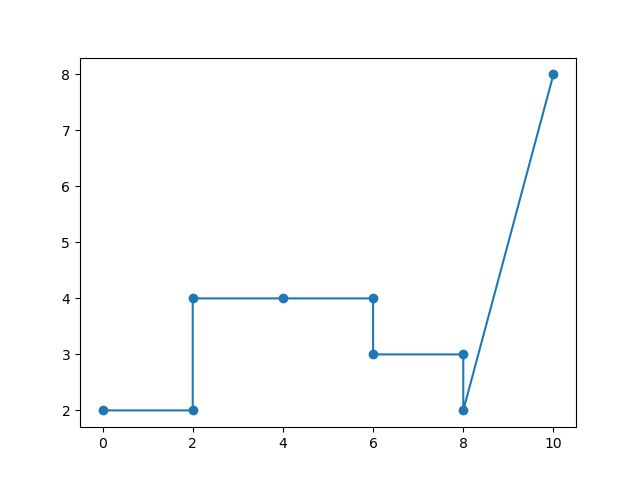
\includegraphics[width=0.5in]{plot.png}
\caption{\label{FIG:fig2}Reconstruct signal \(y(t)\).}
\end{figure}

\subsection{Inline Equation}
\label{sec-1-3}
Consider the differential equation given below.
\aDE{1.5}{1.5}{3.6}{eq2}
\begin{itemize}
\item Find an integral form solution for Eq.\ref{eq2}.
\item Find an analytic solution for Eq.\ref{eq2} when the input \(u(t)\) is  given as , for \(t\ge 0\). Is this input able to stabilize state \(y(t)\) when \( t\rightarrow  \infty\)?
\item Find the difference equation when sampleo time is \(\triangle t=0.3\) by exact discretization.
\item Find the difference equation with time derivative approximated at \(\triangle t=0.3\) by finite difference method.
\item Find a solution of difference equation and exact diference equation using  MATLAB or any other software for \(k=20\).  Plot the sequence of numbers obtained by the exact difference equation and by finite difference method and applied piecewise constant input given as follows
\[ \begin{array}{c} u(0) = -2 \\u(1\triangle t) = -2e^{-2*1\triangle t} \\ u(2\triangle t) = -2e^{-2*2\triangle t} \\ \cdots=\cdots \\ u(k\triangle t)= -2e^{-2*k\triangle t}\end{array} \]

with k=20

Solution:
\end{itemize}







\begin{itemize}
\item \[y(t)=5e^{2t}+1.5e^{2t}\int_0^t (-2) e^{-2s}e^{-2s}ds= 5e^{2t}-3e^{2t} \int_0^t e^{-4s}ds=5e^{2t}-3\int_0^t e^{-4s}\frac{d(-4s)}{-4} \]
       \[y(t)=5e^{2t}+\frac{3}{4}\left[e^{-4t}-1\right]\]
\item Exact discretization \(\Delta t = 0.3\):
\[\begin{array}{rcl}
       y_{k+1} &=& e^{a\Delta t}y_{k} + a^{-1}(e^{a\Delta t}-1)bu_{k} \\[0.25cm]
       &=& 1.822y_{k} + 0.6166u_{k}
       \end{array}\]

\item Finite difference method \(\Delta t=0.3\):
\[\begin{array}{rcl}  \frac{dy}{dt} \approx \frac{y_{k+1}-y_{k}}{\Delta t} &=& 2y_{k} + 1.5u_{k} \\[0.25cm]
         y_{k+1} &=& (1+2\Delta t)y_{k} + 1.5(\Delta t )u_{k} \\[0.25cm]
         &=& 1.6y_{k} + 0.45u_{k}
         \end{array}\]
\end{itemize}

\begin{figure}[!htpb]
\centering
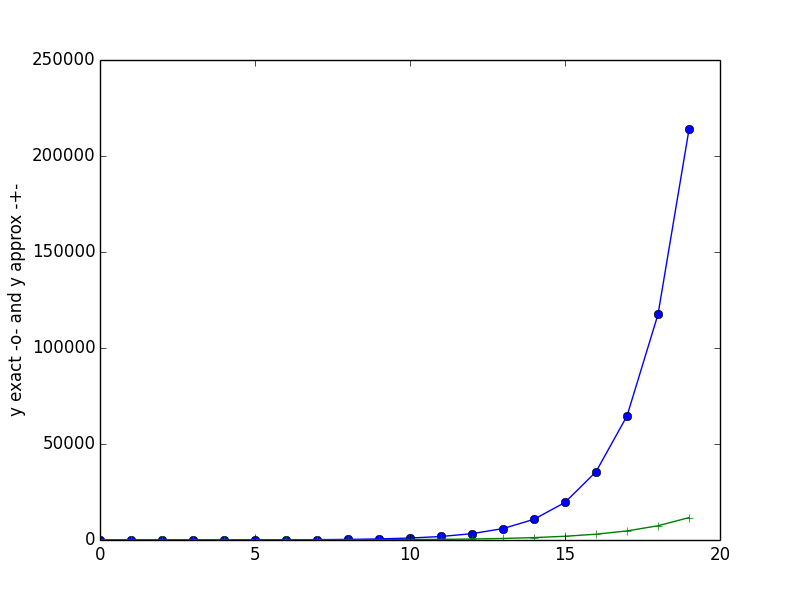
\includegraphics[width=4in]{plot1.png}
\caption{\label{FIG:fig3}Finite difference and exact discretization \(y(k)\).}
\end{figure}



\subsection{ditaa \& \LaTeX{} Graph}
\label{sec-1-4}
For the physical process of tank dynamics given in the Figure below:

\vspace{0.2in}
\setlength{\unitlength}{1cm}
\begin{picture}(1, 1)
  \put(5, 0.9){\vector(1, 0){1.8}}
  \put(6.8, 0.9){\vector(0,-1){0.7}}
  \put(5.5,1.1){{$f_{in}(t)$}}   
  \put(6.3, 0.25){\line(0,-1){1.9}}
  \put(8.2, 0.25){\line(0,-1){1.9}}
  \put(6.3,-1.95){\framebox(1.9,1.9)}
  \put(8., -1.95){\vector(1,0){2.5}}  
  \put(9.6, -2.1){\line(0,0){0.4}}  
  \put(9.3, -2.1){\line(0,0){0.4}}  
  \put(9.3, -2.1){\line(3,4){0.3}}  
  \put(9.3, -1.75){\line(3,-4){0.3}}  
  \put(9.45,-2.){\line(0,1){0.5}}
  \put(9.15,-1.5){\line(1,0){0.5}}
   \put(10.7,-2){{$f_{out}(t)$}}  
   \put(9.3,-1.25){{$K$}}  
    \put(5.5,-1.25){{$h(t)$}}  
\end{picture}
\vspace{0.7in}


Solution:
\begin{itemize}
\item \( \frac{dh}{dt} = -\frac{1}{K\overline{A}}h + \frac{1}{\overline{A}}f_{in}\)
\item Assume that the tank height is measured, \(y(t) = h(t)\)
       \[\Sigma(A,B,C,D) = \Sigma\left(-\frac{1}{K\overline{A}}, \frac{1}{\overline{A}}, 1, 0\right)\]
\item The state-space realization is given as:
\end{itemize}

\begin{figure}[!htpb]
\centering
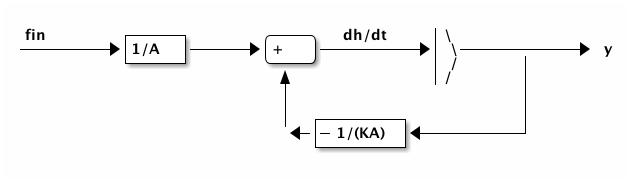
\includegraphics[width=3in,height=1.5in]{hello.png}
{\caption{Block diagram elements.}}
\end{figure}

\begin{itemize}
\item \[\begin{array}{c}
        \Phi = e^{-\frac{0.2}{K\overline{A}}}, \quad \Gamma = -K\left(e^{-\frac{0.2}{K\overline{A}}} - 1\right), \quad \theta = 1 \\[0.5cm]
        \Sigma(A_{d},B_{d},C_{d},D_{d}) = \Sigma\left( e^{-\frac{0.2}{K\overline{A}}}, -K\left(e^{-\frac{0.2}{K\overline{A}}} - 1\right), 1, 0\right)
        \end{array}\]
\item Assume that \(h(0) = 0\). Laplace transform:
\[ \frac{Y(s)}{U(s)} = \frac{5}{s+1}\]
\[\boxed{ \nonumber  \tau = 1, \quad \tau_{d} = 0\Rightarrow \Delta t = (0.1\sim0.2)1\tau = 0.1\sim 0.2}\]
\end{itemize}

\begin{minted}[]{elisp}
(expand-file-name
	     "ditaa.jar"
      (file-name-as-directory
	    (expand-file-name
		"scripts"
	       (file-name-as-directory
		  (expand-file-name
		      "../contrib"
		     (file-name-directory (org-find-library-dir "org")))))))
\end{minted}
% Emacs 25.3.1 (Org mode 8.2.10)
\end{document}
